\chapter{The Impact of Genetic Drift on Selected Alleles}
\label{Selection_Stochasticity}
%\begin{quote}
%``Did he fire six shots or only five? [...] you've got to ask yourself
%one question'' `Do I feel lucky?' Well do ya, punk? '' -- Dirty Harry 
%\end{quote}

In the previous chapter we assumed that the selection acting on our
alleles was strong enough that we could ignore the action of genetic
drift in shaping allele frequencies. However, genetic drift affects all
alleles, and so in this chapter we explore the interaction of
selection and drift. Strongly selected alleles can be
lost from the population via drift when they are rare in the population, while both weakly
beneficial and weakly deleterious alleles are subject to the random
whims of genetic drift throughout their entire time in the
population. Understanding the interaction of selection and genetic
drift is key to understanding the extent to which small populations
may be mutation-limited in their rates of adaptation, and how rates of
molecular and genome evolution may differ across taxa.
%In Chapter \ref{Chapter:Drift}

\section{Stochastic loss of strongly selected alleles}

% Fisher (1922, 1930) and Haldane (1927)
Even strongly beneficial alleles can be lost from the population when
they are sufficiently rare. This is because the number of offspring
left by individuals to the next generation is fundamentally
stochastic. A selection coefficient of s=$1\%$ is a strong
selection coefficient, which can drive an allele through the
population in a few hundred generations once the allele is
established. However, if individuals have on average a small number of
offspring per generation, the first individual to carry our beneficial allele, who
has on average $1\%$ more children than their peers, could easily have zero offspring, leading to the loss
of our allele before it ever gets a chance to spread.\\

To take a first stab at this problem, let's think of a very large
haploid population in which a single individual starts with the selected allele, and ask
about the probability of eventual loss of our selected allele starting
from this single copy. To derive this probability of loss ($p_L$), we'll make use of a
simple argument \citep[derived from branching processes][]{fisher1923xxi,haldane1927mathematical}. Our selected
allele will be eventually lost from the population if every individual
with the allele fails to leave descendants.
\begin{figure*}
\begin{center}
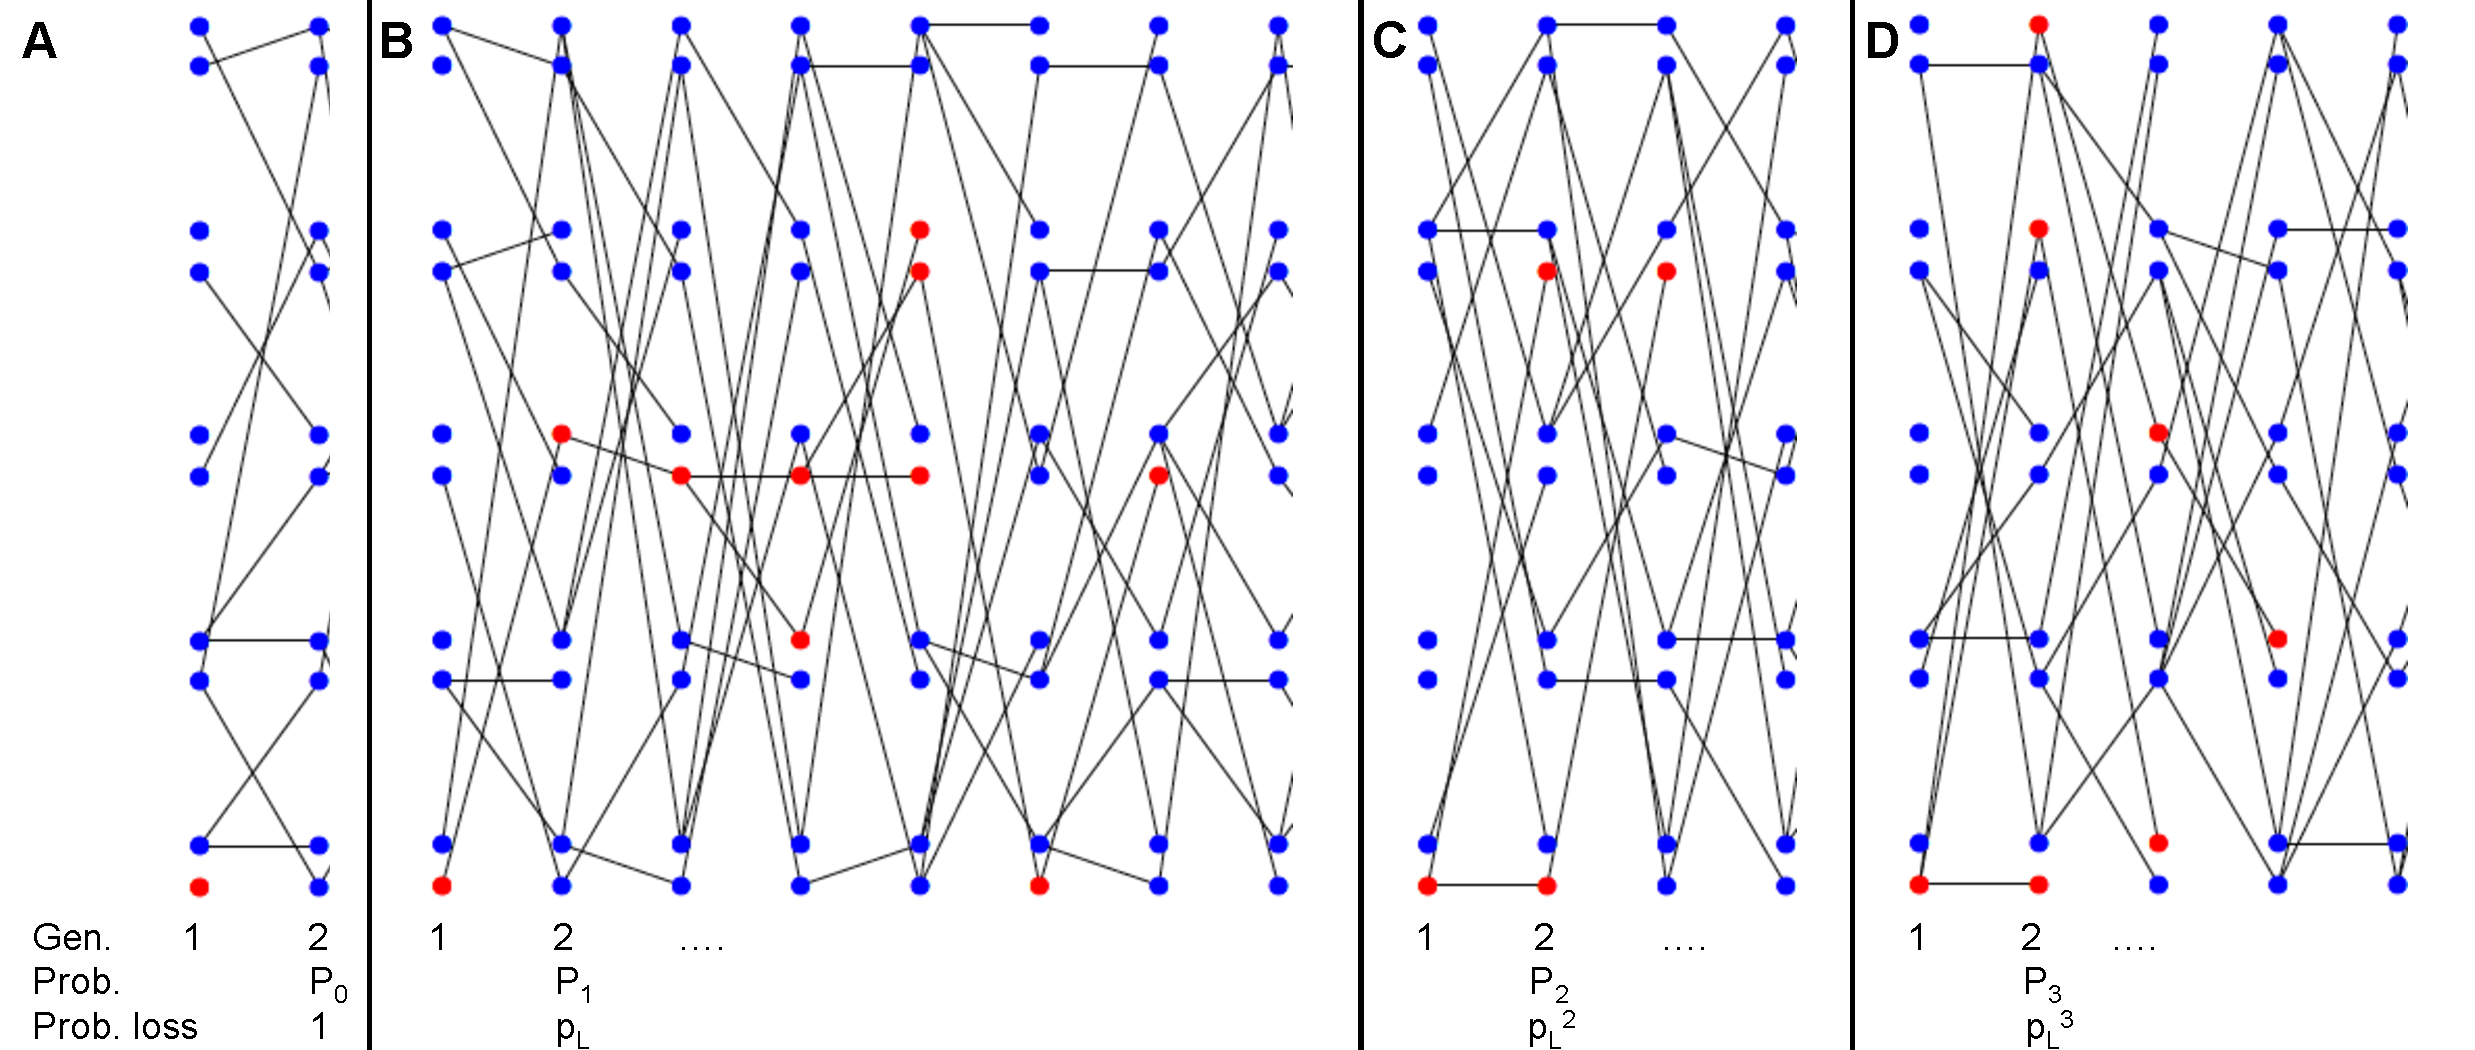
\includegraphics[width=0.9 \textwidth]{figures/Proof_of_pL_2s.pdf}
\end{center}
\caption{} \label{fig:Proof_of_pL_2s}
\end{figure*}
Well we can think about different cases: 
\begin{enumerate}
\item In our first generation,
with probability $P_0$ our individual allele leaves no copies of itself to
the next generation, in which case our allele is lost (Figure \ref{fig:Proof_of_pL_2s}A).
\item Alternatively,
our allele could leave one copy of itself to the next generation (with
probability $P_1$), in which
case with probability $p_L$ this copy eventually goes extinct (Figure \ref{fig:Proof_of_pL_2s}B).
\item Our allele could leave two copies of itself to the next generation (with
probability $P_2$), in which
case with probability $p_L^2$ both of these copies eventually go
extinct (Figure \ref{fig:Proof_of_pL_2s}C).
\item More generally, our allele could leave could leave $k$ copies ($k>0$) of itself to the next generation (with
probability $P_k$), in which case with probability $p_L^k$  all of
these copies eventually go extinct (e.g. Figure \ref{fig:Proof_of_pL_2s}D).
\end{enumerate}
Summing over these probabilities, we see that
\begin{equation}
  p_L = \sum_{k=0}^{\infty} P_k p_L^{k}
\end{equation}
We'll now need to specify $P_k$, the probability that an individual
carrying our selected allele has $k$ offspring. In order for this population to stay constant in size,
we'll assume that individuals without the selected mutation have on average one
offspring per generation, while individuals with our selected allele
have on average $1+s$ offspring per generation. We'll assume that the
number of offspring an individual has is Poisson
distributed with mean given by $1$ or $1+s$, i.e. the probability that an individual
with the selected allele has $i$ children is
\begin{equation}
P_i= \frac{(1+s)^i e^{-(1+s)}}{i!}
\end{equation}
Substituting $P_k$ into the equation above, we see
  \begin{align}
p_L &=  \sum_{k=0}^{\infty} \frac{(1+s)^ke^{-(1+s)}}{k!} p_L^{k} \nonumber
\\
&= e^{-(1+s)} \left( \sum_{k=0}^{\infty} \frac{\left(p_L(1+s) \right)^k}{k!}  \right)
\end{align}
The term in the brackets is itself an exponential expansion, so
we can rewrite this equation as
\begin{equation}
p_L = e^{(1+s)(p_L-1)} \label{prob_loss}
\end{equation}
Solving for $p_L$ would give us our probability of loss for any selection
coefficient. Let's
rewrite our result in terms of the the probability of escaping loss, $p_F = 1-p_L$.  We can
rewrite eqn. \eqref{prob_loss} as
\begin{equation}
1-p_F = e^{-p_F(1+s)}
\end{equation}
To gain an approximate solution for this result, let's consider a small selection
coefficient $s \ll 1$ such that $p_F \ll 1$ and {then use a Taylor series to expand out the
exponential on the right hand side (ignoring terms of higher
order than $s^2$ and $p_F^2$):
\begin{equation}
1-p_F \approx 1-p_F(1+s)+p_F^2(1+s)^2/2
\end{equation}
Solving this we find that
\begin{equation}
p_F = 2s.
\end{equation}
Thus even an allele with a $1\%$ selection coefficient has a $98\%$
probability of being lost when it is first introduced into the
population by mutation. \\

If the mutation rate towards our advantageous allele is $\mu$, and there
are $N$ individuals in our haploid population, then $N \mu$ advantageous mutations
arise per generation.  Each of these new beneficial mutations has a probability $p_F$ of
fixing. Thus the number of advantageous mutations
arising per generation that will eventually fix in the population is $N \mu p_F$, and
the waiting time for a mutation that will fix to arise is the reciprocal of
this: $\nicefrac{1}{N\mu p_F}$. Thus, in adapting to a novel selection
pressure via new mutations, the population size, the mutational
target size, and the selective advantage of new mutations all matter. One reason why combinations of drugs
are used against viruses like HIV and malaria is that, even if the viruses adapt to one
of the drugs, the viral load ($N$) of the patient is greatly reduced, making it very
unlikely that the population will manage to fix a second drug-resistant allele.

\paragraph{Diploid model of stochastic loss of strongly selected alleles.}
%%consider reparameterizing 1+(1-hs)s
We can also adapt this result to a diploid setting.
Assuming that heterozygotes for the $1$ allele have on average $1+hs$ children, the
probability allele $1$ is not lost, starting from a single copy in
the population, is
\begin{equation}
p_F = 2 h s \label{eqn:diploid_escape}
\end{equation}
for $h>0$. Note this is a slightly different parameterization from
our diploid model in the previous chapter; here $h$ is the dominance of our positively selected
allele, with $h=1$ corresponding to the full selective advantage expressed in an individual with only a single copy. Thus the probability that a beneficial allele is not lost depends just
on the relative fitness advantage of the heterozygote; this is because
when the allele is rare it is usually present in heterozygotes and so
its probability of escaping loss just depends on the fitness of these
individuals compared to homozygotes for the ancestral allele (assuming an
outbred population). \\

\begin{figure}
\begin{center}
  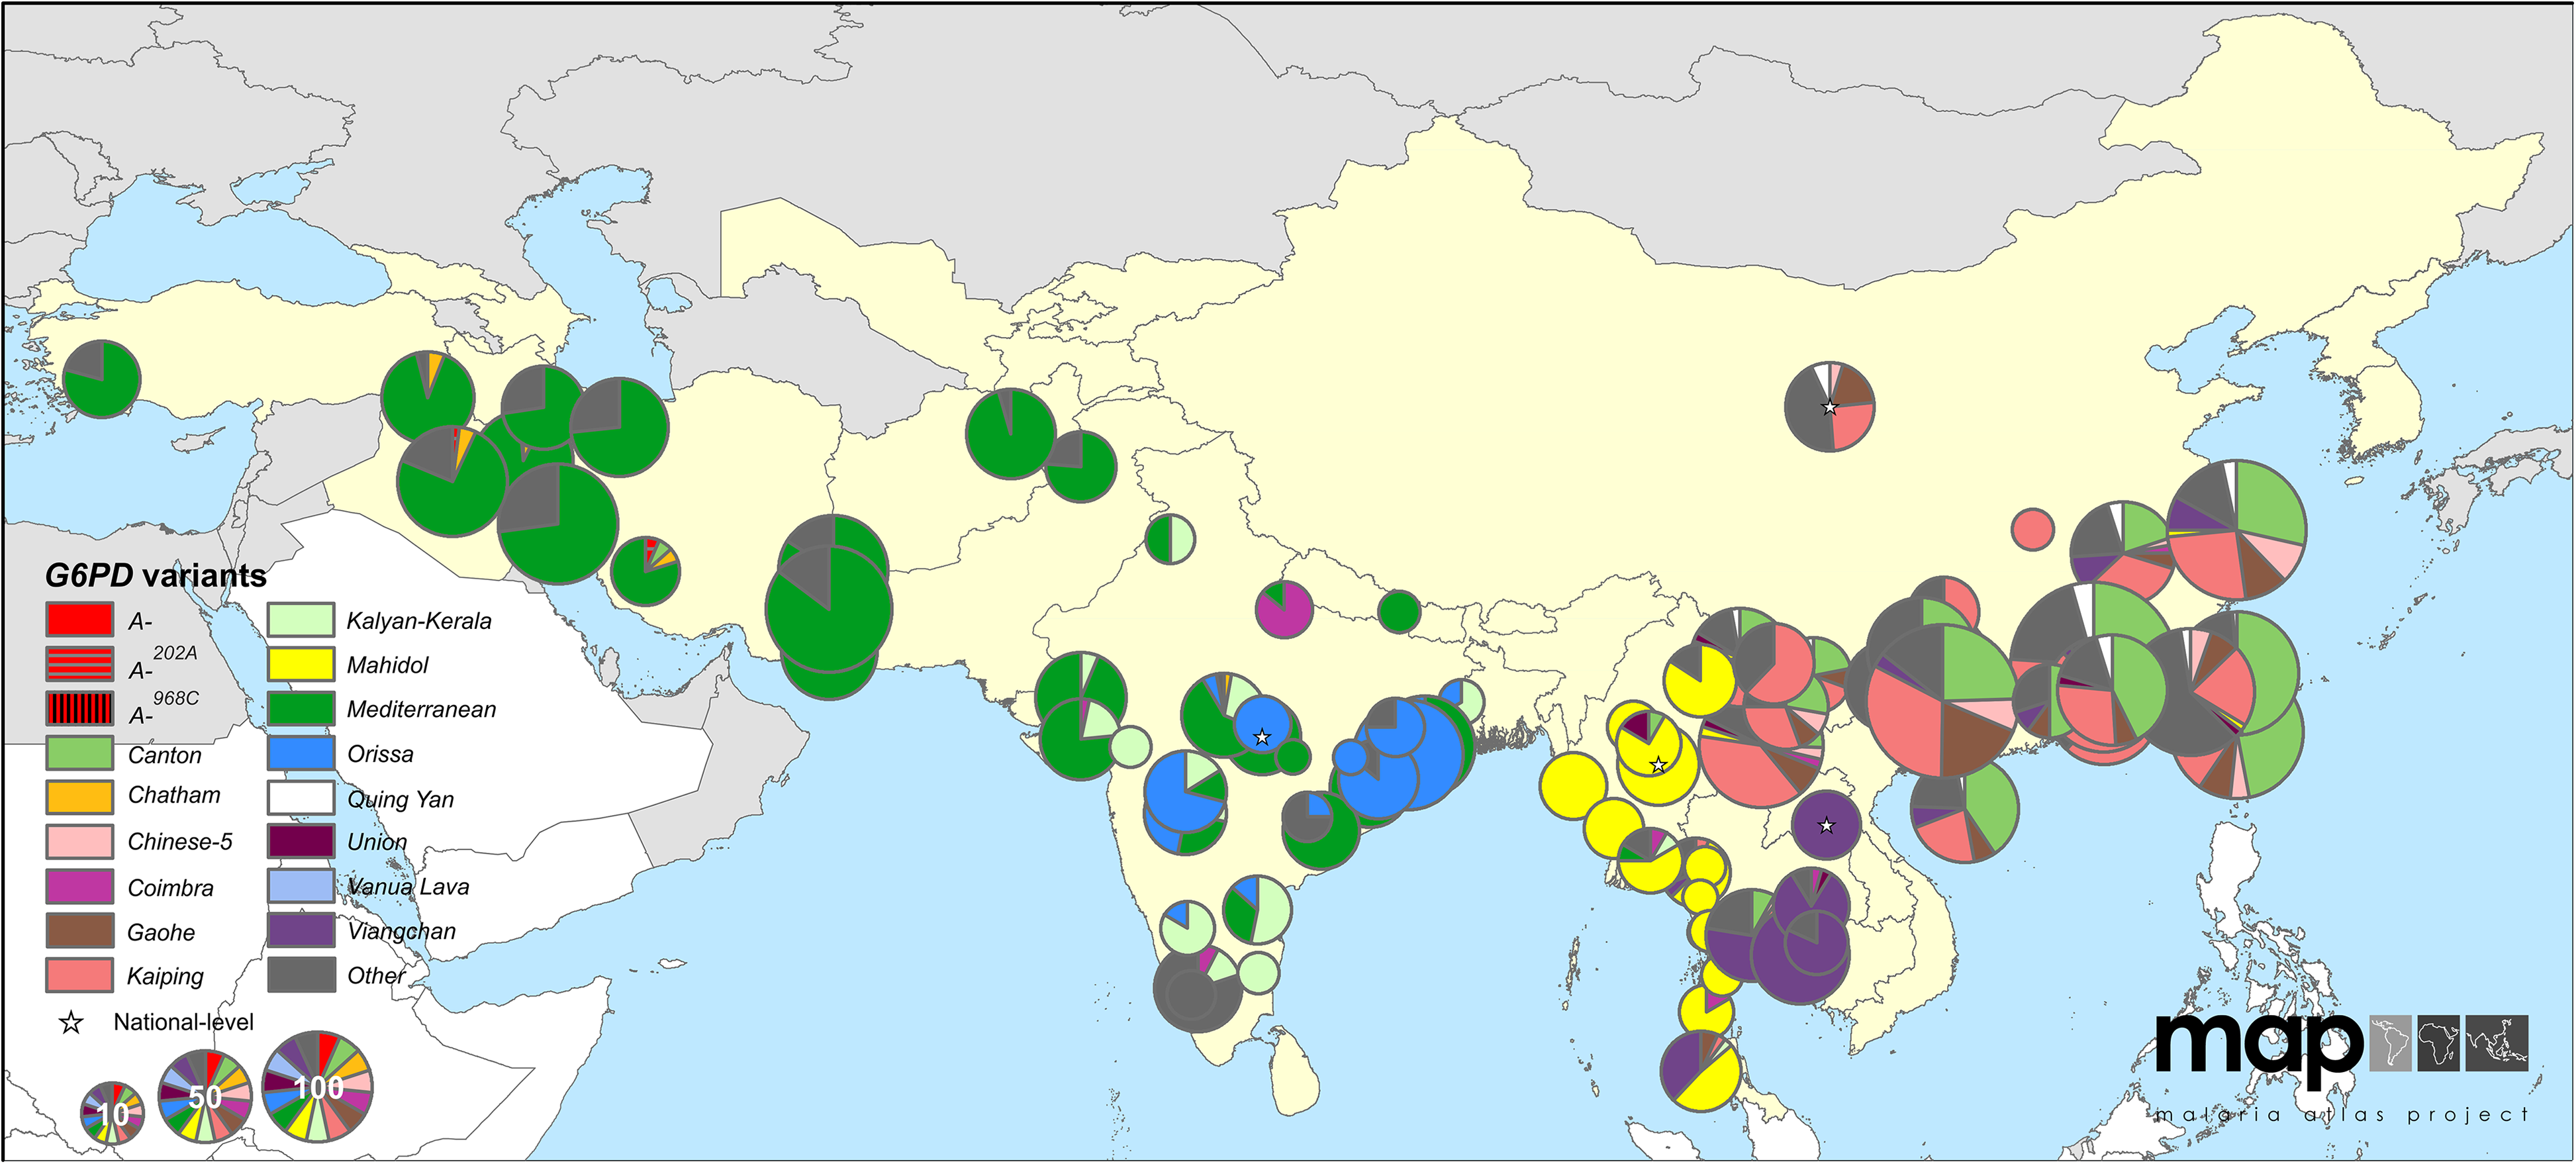
\includegraphics[width=0.9 \textwidth]{Journal_figs/drift_selection/G6PD/G6pd_Howes_et_al_1475-2875-12-418-4.png} 
\caption{ 
{\bf Map of G6PD-deficiency allele frequencies across Asia.} 
The pie chart shows the frequency of G6PD-deficiency alleles. 
The size of the pie chart indicates the number of G6PD-deficient individuals sampled.
Countries with endemic malaria are colored yellow. 
Figure taken from \citet{Howes-g6pd-variants}
\url{http://www.malariajournal.com/content/12/1/418}. 
} \label{fig-G6PD-map}
\end{center}
\end{figure}

Over roughly the past ten thousand years, adaptive alleles conferring resistance to malaria have arisen in a number of genes 
and spread through human populations in areas where malaria is endemic
\citep{Kwiatkowski:05}. One particularly impressive case of convergent evolution in response to
selection pressures imposed by malaria are the numerous changes
throughout the G6PD gene,
which include at least 15 common variants in Central and Eastern Asia alone that lower the activity of the
enzyme \citep{Howes-g6pd-variants}. 
These alleles are now found at a combined frequency of around 8\% frequency in malaria endemic areas,
rarely exceeding 20\% \citep{Howes-g6pd-preval}. Whether these variants {\it all} confer resistance to malaria is unknown,
but a number of these alleles have demonstrated effects against
malaria and are thought to have a selective advantage to heterozygotes $sh > 5\%$ where malaria is endemic \citep{Ruwende-g6pd,tishkoff-g6pd,Louicharoen-g6pd}. 

With a 5\% advantage in heterozygotes, a G6PD allele present as a
single copy would only have a 10\% probability of
fixing in the population. If that's so, how come malaria adaptation has
repeatedly occurred via changes at G6PD? Well, maybe adaptation didn't
start from a single copy of the selected allele. How many copies of
the G6PD-deficiency alleles do we expect were segregating in the population before
selection pressures changed? 
\begin{marginfigure}
\begin{center}
  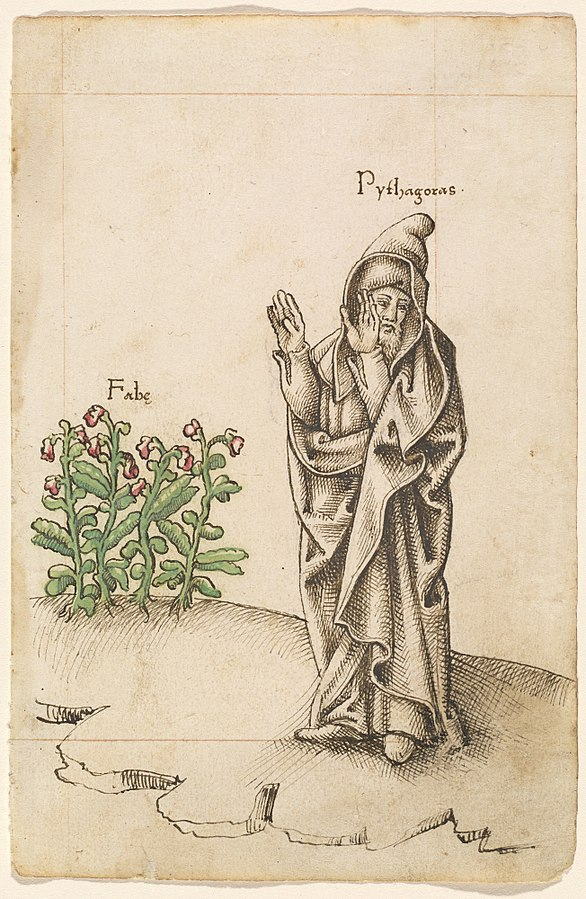
\includegraphics[width=\textwidth]{illustration_images/Genetic_drift_selection/Pythagoras_fava_beans/586px-Do_Not_Eat_Beans.jpg}
\caption{
Pythagoras's ``just say no to fava beans'' campaign. French early 16th Century. Woodner Collection, National Gallery of Art.
Pythagoras prohibited the consumption of fava beans by his followers; perhaps because favaism, the anemia induced in G6PD-deficient
individuals by fava beans, is relatively common in the Mediterranean due
to adaptation to endemic malaria. } \label{fig:fava}
\end{center}
\end{marginfigure}

In the absence of malaria, these G6PD alleles are deleterious with
carriers suffering from G6PD deficiency,
leading to hemolytic anemia when individuals are exposed to a variety of different compounds, notably those present in fava beans.
There's upward of one hundred bases where G6PD-deficiency alleles can arise, so assuming a mutation rate of $\approx 10^{-8}$ per base pair per
generation, we can roughly estimate the rate of mutations arising that affect the G6PD gene as $\mu \approx
10^{-6}$ per generation. In the absence of malaria, the selective cost of being a heterozygotes carrier of a G6PD-deficient allele must have been on the order of
$5\%$ or more, and thus the frequency of the allele under
mutation-selection balance would have been $\approx \nicefrac{10^{-6}}{0.05} =2
\times 10^{-5}$. Assuming an effective population size of  $2-20$ million
individuals, roughly five to ten thousand years ago that means that
there would have been forty to four hundred copies of the G6PD-deficiency
allele present in the population when selection pressures shifted at the introduction of malaria. The
chance that one of these newly adaptive alleles is lost
is $90\%$ but the chance that they're all lost is $<(0.9)^{40}\approx 0.02$, i.e. there would have been a
greater than $98\%$ chance that adaptation would occur via one or more
alleles at G6PD. How many alleles would escape drift? Well with $40 - 400$
copies of the allele pre-malaria, and each of them having a $10\%$
probability of escaping drift, we expect between $4$ and $40$ G6PD
alleles to escape drift and contribute to adaptation. We see $15$ common G6PD
alleles in Eurasia, so our simple model of adaptation from
mutation-selection balance seems reasonable.  \marginnote{A full
  analysis of this case requires modeling of G6PD's X chromosome
  inheritance, and the randomness in the number of copies of the
  allele present at mutation-selection balance \citep{ralph2015role}.} 

\begin{marginfigure}
  \begin{center}
    
\includegraphics[width=0.6\textwidth]{figures/haldanes_sieve.png}
\end{center}
\caption{Haldane's sieve. To our knowledge Haldane never wore a sieve, but we assume he owned one.} \label{fig:haldanes_sieve}
\end{marginfigure}

\begin{question}
`Haldane's sieve' is the name for the idea that the mutations that contribute to adaptation are likely to be dominant or at least co-dominant. \\
{\bf A)} Briefly explain this argument with a verbal model relating to the
results we've developed in the last two chapters. \\
{\bf B)} Haldane's sieve is thought to be less important for adaptation from previously deleterious standing variation, than adaptation from new mutation. Can you explain the intuition behind of this idea?\\
{\bf C)} Haldane's sieve is likely to be less important in inbred,
e.g. selfing, populations. Why is this? \\

\end{question}

\begin{question}
Melanic squirrels suffer a higher rate of predation (due to hawks) than normally pigmented squirrels. Melanism is due to a dominant, autosomal mutation. The frequency of melanic squirrels at birth is $4 \times 10^{-5}$.\\

{\bf A)} If the mutation rate to new melanic alleles is $10^{-6}$, assuming the melanic allele is at mutation-selection equilibrium, what
is the reduction in fitness of the heterozygote? \\ 
Suddenly levels of pollution increase dramatically in our population,
and predation by hawks now offers an equal (and opposite) advantage to
the dark individuals as it once offered to the normally pigmented
individuals. \\
{\bf B)} What is the probability that a single copy of this allele
(present just once in the population) is lost?\\ 
{\bf C)}  If the population size of our squirrels is a million
individuals, and is at mutation-selection balance, what is the probability that the population adapts from one or more allele(s) from the standing pool of melanic alleles?  
\end{question}


\section{The interaction between genetic drift and weak selection.}
 \begin{marginfigure}
 \begin{center}
 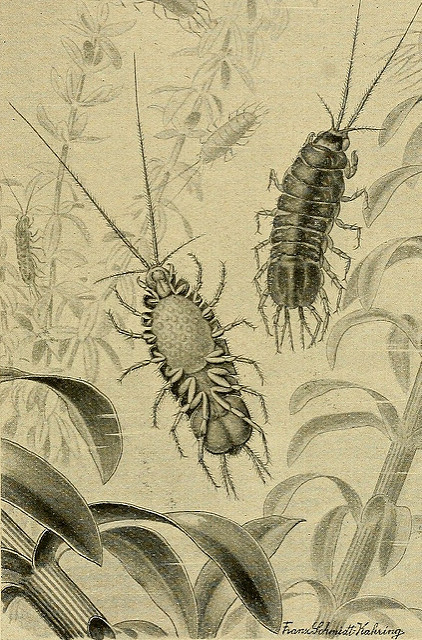
\includegraphics[width=0.7 \textwidth]{illustration_images/Genetic_drift_selection/Isopod_Asellidae/20406697312_1a9aa75024_z.jpg}
 \end{center}
 \caption{cress bug ({\it Asellus aquaticus}) in the isopod family
   {\it Asellidae}. Brehms Tierleben. Allgemeine kunde des Tierreichs (1911).  Brehm A.E.} \label{fig: asellid_isopod}
 \end{marginfigure}
For strongly selected alleles, once the allele has escaped initial
loss at low frequencies, its path will be determined deterministically by its
selection coefficients. However, if selection is weak compared to
genetic drift, the stochasticity of reproduction can play a role in the trajectory an
allele takes even when it is common in the population. If selection is
sufficiently weak compared to genetic drift, then genetic drift will dominate the dynamics of alleles
and they will behave like they're effectively neutral. Thus, the extent
to which selection can shape patterns of molecular evolution will
depend on the relative strengths of selection and genetic drift.
But how weak must selection on an allele be for drift to overpower
selection? And do these interactions between selection and drift have longterm consequences for genome-wide patterns evolution?

 \begin{marginfigure}
 \begin{center}
 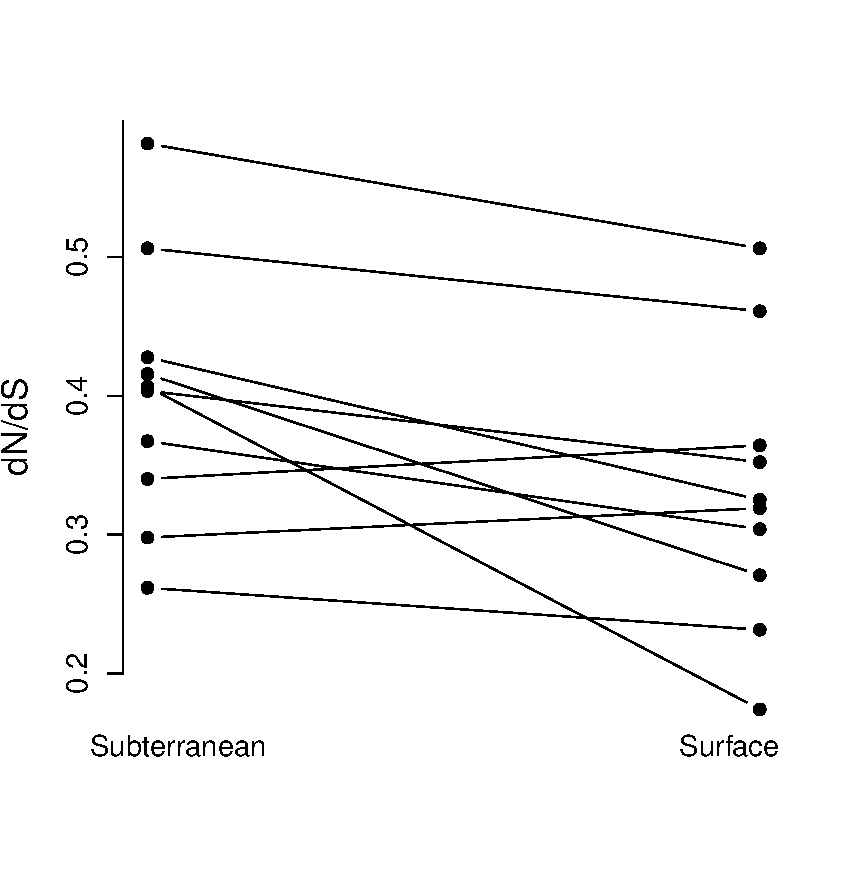
\includegraphics[width=\textwidth]{Journal_figs/drift_selection/asellid_isopods_Nes/asellid_isopods_Nes.pdf}
 \end{center}
 \caption{ Asellid isopods have repeatedly invaded subterranean, ground-water
habitats from surface-water habitats, and leading to a
genome-wide increase in $\dNdS$  and larger genomes \citep[Figure from ][comparing independent isopod species pairs]{lefebure2017less}. One
possible explanation of this is that the longterm effective population
sizes of the subterranean species are lower and so these species are less able to
prevent mildly deleterious alleles fixing, and also less able to prevent genome expansion from the accumulation of weakly deleterious, extraneous
genomic DNA. } \label{fig: asellid_isopods_Nes}
 \end{marginfigure}


% \begin{figure}
% \begin{center}
% 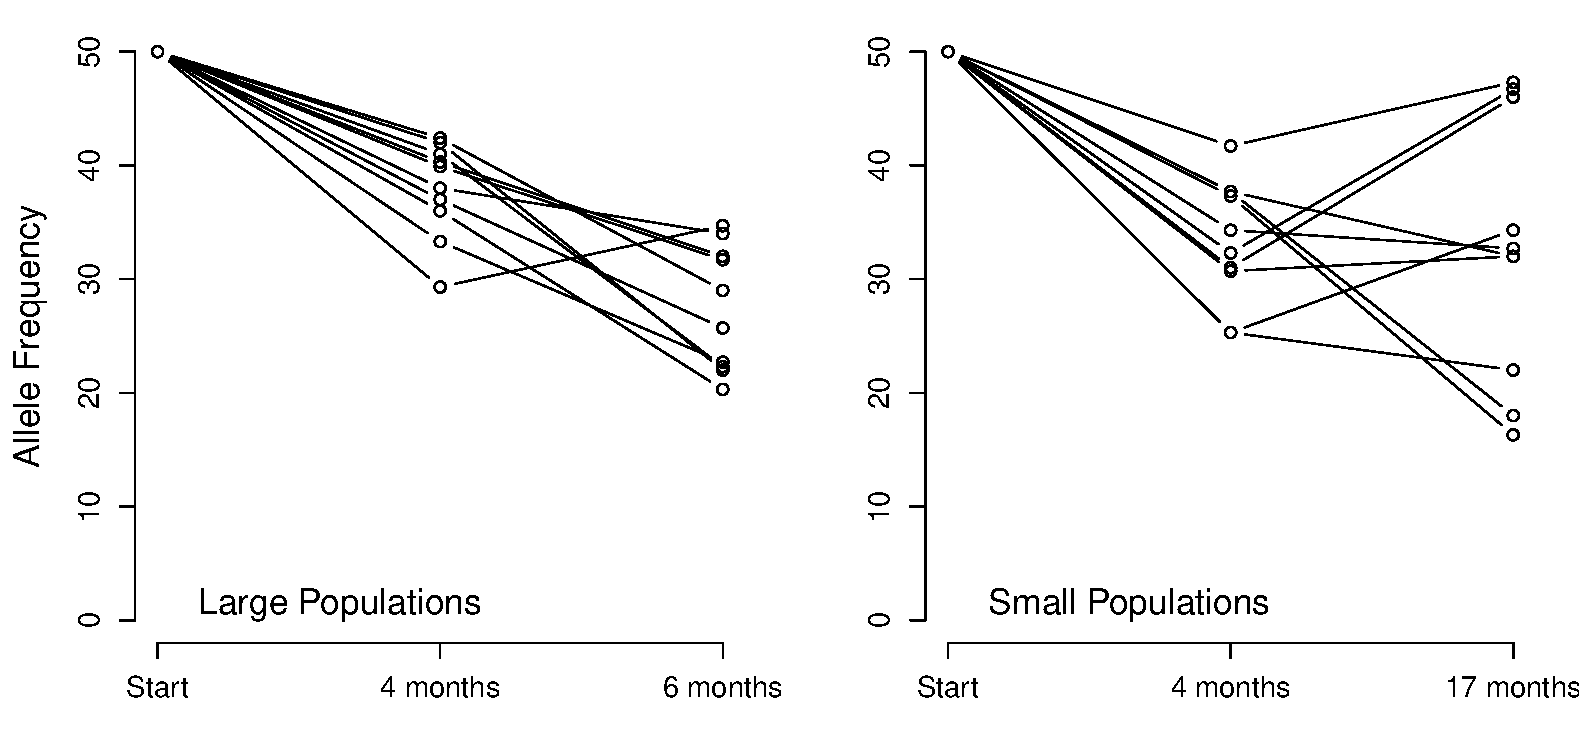
\includegraphics[width=\textwidth]{Journal_figs/drift_selection/DobPav/Drift_sel_Dobzhansky_Pavlovsky.pdf}
% \end{center}
% \caption{Data from \citet{dobzhansky1957experimental} } \label{fig:Dobzhansky_Pavlovsky}
% \end{figure}
% A classic case study of the interplay of genetic drift with selection is the
%  {\it Drosophila pseudoobscura} experiments of
% \citet{dobzhansky1957experimental}. \citeauthor{dobzhansky1957experimental} 
% setup multiple large populations each with 4000 indviduals and
% multiple small populations of 20
% individuals. They initiated each of these populations with the `Pikes
% Peak' (PP) inversion allele at $50\%$
% frequency.
% The PP allele was known to experience heterozygote advantage, with the
% PP homozygotes being less fit than the alternate homozygotes. In all of the
% large population cages moved relatively uniformly towards the
% equilbrium frequency. However, due to geneti drift in  

%To see this lets think of our simple Wright-Fisher model (see R
%exercise).

 To model selection and drift each generation, we can first calculate the deterministic change in our
allele frequency due to selection using our deterministic formula.  Then, using our newly calculated expected allele frequency, we can binomially sample two alleles for each of our offspring to construct the next generation. This approach to jointly modeling genetic drift and selection is called the Wright-Fisher model. 
%%%%%Include this discussion of sampling back in our HWE section??
%%%%%Next time

Under the Wright-Fisher model, we will calculate the expected change in allele frequency due to selection and the variance around this expectation due to drift. To make our calculations simpler, let's assume an additive model, i.e. $h=1/2$, and that $s \ll 1$ so that $\wbar
\approx 1$. Using our directional selection deterministic model, from Chapter
\ref{Chapter:OneLocusSelection}, and these approximations gives us our deterministic change due to selection
\begin{equation}
\Delta_S p = \E(\Delta p) = \frac{s}{2} p(1-p) \label{eqn:WF_mean}
\end{equation}
To obtain our new frequency in the next generation, $p_1$, we binomially sample from our new deterministic frequency $p^{\prime}= p + \Delta_S p$,
so the variance in our allele frequency change from one generation to the next is given by
\begin{equation}
Var(\Delta p) = Var(p_1 - p) = Var(p_1) = \frac{p^{\prime}(1-p^{\prime})}{2N} \approx  \frac{p(1-p)}{2N}. \label{eqn:WF_var}
\end{equation}
\marginnote{To see this denote our new count of allele $1$ by $i$, then
\begin{eqnarray}
\textrm{Var} (p_1 - p)  = &\textrm{Var} (\frac{i}{2N} - p) = \textrm{Var} (\frac{i}{2N} )\nonumber\\ 
= &  \frac{\textrm{Var} (i)}{(2N)^2} \nonumber
\end{eqnarray}
and from binomial sampling $\textrm{Var} (i) = 2N p^{\prime}(1-p^{\prime})$ and
so we arrive at our answer. Assuming that $s \ll 1$, $p^{\prime}
\approx p$, then in practice we can use
\begin{equation}
\textrm{Var} (\Delta p)  =\textrm{Var} (p^{\prime} - p) \approx \nicefrac{p(1-p)}{2N}. \nonumber
\end{equation} }
where the previous allele frequency $p$ drops out because it is a constant and the variance in our new allele frequency follows from the fact that we
are binomially sampling $2N$ new alleles from a frequency $p^{\prime}$ to form the next
generation. 

To get our first look at the relative effects of selection vs. drift we
can simply look at when our change in allele frequency caused by
selection within a generate is reasonably faithfully passed down through the generations. In particular, if our expected change in allele frequency is much greater than the variance around this change, genetic drift will play little role in the fate of our selected allele (once the allele is not at low copy number within the population). When does selection dominant genetic drift? This will happen if $\E(\Delta p) \gg Var(\Delta p)$, i.e. when $|Ns| \gg 1$. Conversely, any hope of our selected allele following its deterministic path will be quickly undone if our change in allele frequencies due to selection is
much less than the variance induced by drift. So if the absolute value of our population-size-scaled selection coefficient $| Ns| \ll 1$, then drift will dominate the fate of our allele. \\
\begin{figure}
\begin{center}
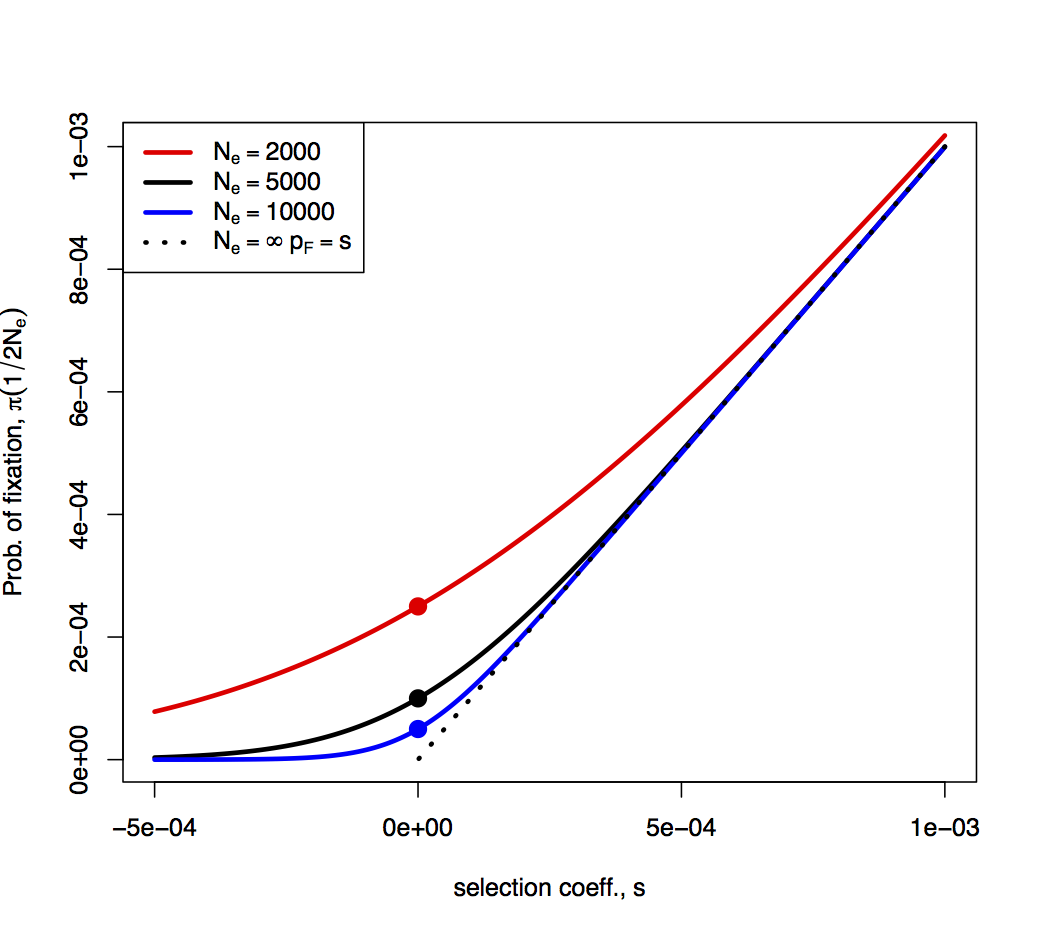
\includegraphics[width=0.9 \textwidth]{figures/prob_fix_diffusion.png}
\end{center}
\caption{The probability of the fixation of a new mutation with
  selection coefficient $s$ ($h=1/2$) in a diploid population of effective
  size $N_e$. The dashed line gives the infinite population
  solution. The dots give the solution for $s \rightarrow 0$, i.e. the neutral case, where the probability of fixation is $1/(2N_e)$} \label{fig:prob_fix_diffusion}
\end{figure}

To make further progress on understanding the fate of alleles with
selection coefficients of the order $1/N$ requires more careful
modeling. However, under our diploid model, with an additive selection coefficient $s$, we can obtain the probability that allele $1$ fixes within the population, starting
from a frequency $p$ :
\begin{equation}
p_F(p) = \frac{1-e^{-2Ns p }}{1-e^{-2Ns}} \label{eqn:prob_fixed}
\end{equation}
The proof of this result is sketched out below (see Section \ref{Section:fixation_weakly_sel}). A new allele that arrives in the population at frequency $p=1/(2N)$ has a probability of reaching fixation of
\begin{equation}
p_F \left(\frac{1}{2N} \right) = \frac{1-e^{-s }}{1-e^{-2Ns}} \label{eqn:new_mut_prob_fixed}
\end{equation}
If $s \ll1$ but $Ns \gg 1$ then $p_F(\frac{1}{2N}) \approx s$, which
nicely gives
us back the result that we obtained above for an allele under strong selection
(eqn. \eqref{eqn:diploid_escape}). Our probability of fixation
(eqn. \eqref{eqn:new_mut_prob_fixed}) is plotted as a function of $s$
and $N$ in Figure \ref{fig:prob_fix_diffusion}. To recover our neutral
result, we can take the
limit $s \rightarrow 0$ to obtain our neutral fixation
probability, $\nicefrac{1}{(2N)}$. \\

In the case where $Ns$ is close to $1$, then
\begin{equation}
p_F \left( \frac{1}{2N} \right) \approx \frac{s}{1-e^{-2Ns}} \label{eqn:escape_from_intro}
\end{equation}
This is greater than our earlier result $p_F=s$ from the branching process
argument (using our additive model of $h=1/2$), increasingly so for smaller $N$. 
Why is this?  The reason why is that $p_F$ is really the probability
of "never being lost" in an infinitely large population. So to persist
indefinitely, the allele has to escape loss permanently, by never being
absorbed by the zero state. When the population size is finite, to fix
we only need to reach a size 2N individuals. Weakly beneficial
mutations (Ns~1) are slightly more likely to fix than the s
probability, as they only have to reach 2N to never be lost.

If, for selection to operate on an allele, we need the selection coefficient to satisfy
$|Ns|\gg 1$, then that holds if $|s|\gg \nicefrac{1}{N}$. 
Well, effective population sizes are often reasonably large, on the
order of hundreds of thousands or millions of individuals, thus selection
coefficients on the order of $10^{-5}$ to $10^{-6}$ can be effectively selected upon, i.e. selection
equivalent to individuals have incredibly slight advantages in terms
of the number of offspring they leave to the next generation.
While we are incapable of detecting measuring all but the large fitness effect sizes,  
except in some elegant experiments (e.g. in microbes), such small effects are visible to
selection in large populations. Thus, if consistent selection pressures are exerted over long
time periods, natural selection can potentially finely tune various aspects of an organism.

\begin{marginfigure}
\begin{center}
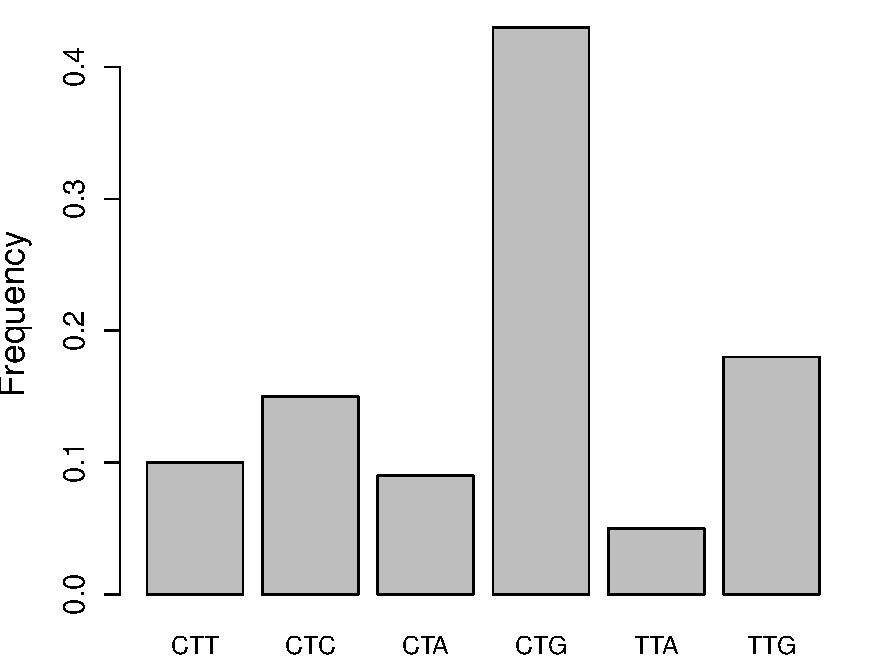
\includegraphics[width=\textwidth]{Journal_figs/drift_selection/Codon_bias_Drosophila/Leucine_codon_bias.pdf}
\end{center}
\caption{Data from {\it Drosophila melanogaster} on the frequency of
  different codons for Leucine.} \label{fig:Leucine}
\end{marginfigure}
As one example of this fine-tuning, consider how carefully crafted and optimized the sequence of codons is for translation. Due to the degeneracy of the protein code, multiple codons code for the same
amino-acid. For example, there are six different codons that can code
leucine. While these synonymous codons are equivalent at the protein
level, cells do differ in the number of tRNA molecules that bind
these codons and so the efficacy and accuracy with which proteins can be formed through
translation and folding.  These slight differences in translation rates
likely often correspond to tiny differences in fitness, but do they
matter?

\begin{marginfigure}
\begin{center}
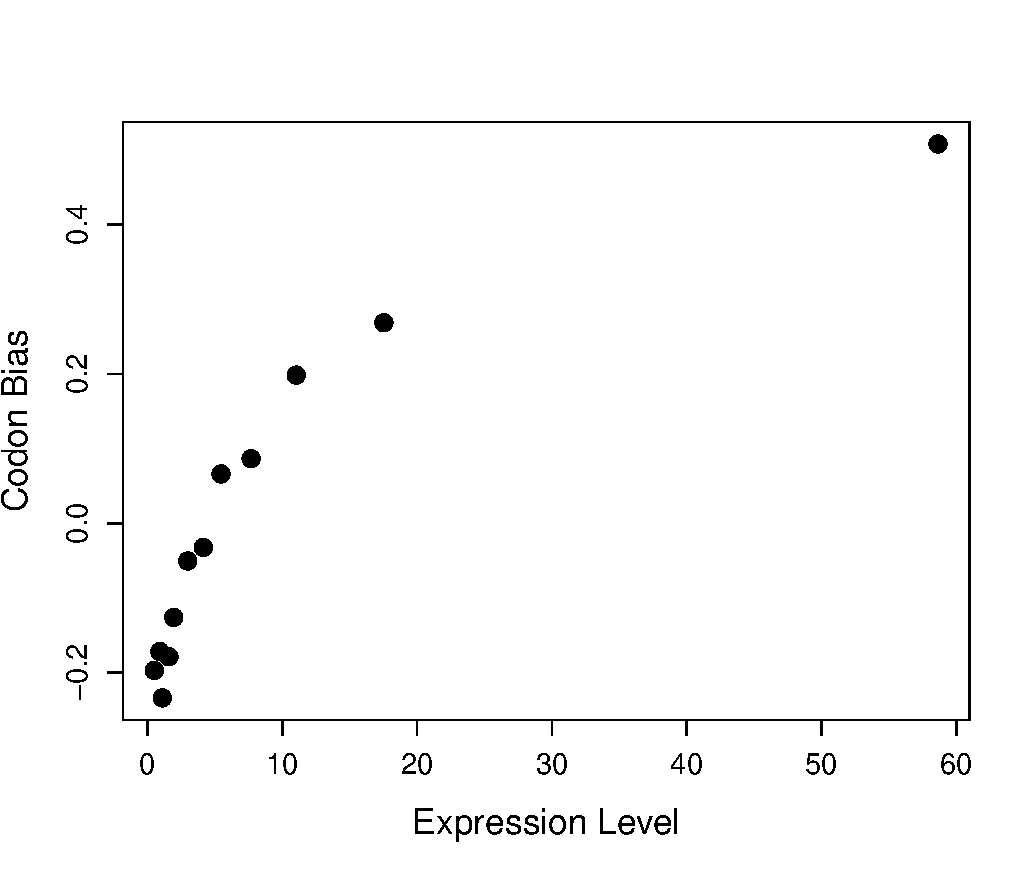
\includegraphics[width=\textwidth]{Journal_figs/drift_selection/Codon_bias_Drosophila/Drosophila_codon_bias_expression.pdf}
\end{center}
\caption{Data from {\it Drosophila melanogaster} on the codon bias for
  different codons for Leucine.} \label{fig:Leucine}
\end{marginfigure}
In many organisms there is a strong bias in the codons to encode
particular amino-acids, see Figure \ref{fig:Leucine}, with the most
abundant codon matching the most abundant tRNA in cells. This 'codon bias' likely reflects the combined action of weak selection and
mutational pressure, pushing the codon composition of the genome and tRNA abundances towards an adaptive compromise. These selection
pressures have acted over long time periods, as codon usage patterns
are often very similar for species that diverged over many tens of millions of years ago. 
Compared to other genes, highly expressed genes show a strong bias towards using
codons matching abundant tRNAs, consistent with the idea that the synonymous codon content of
highly expressed genes is evolving to optimize their
translation. These patterns likely represent the action of
selection pressures that are incredibly weak on average, but that have played out
over vast time-periods. 



%Well in s
%mall populations selected alleles spend a
%somewhat shorter time segregating (especially at low frequencies), and so are
%slightly less susceptible to genetic drift. \\

\paragraph{The fixation of slightly deleterious alleles.}
From Figure \ref{fig:prob_fix_diffusion} we can see that weakly
deleterious alleles can also fix, especially in small populations.  To understand how
likely it is that deleterious alleles by chance reach fixation by
genetic drift, let's assume a diploid model with additive selection (with
a selection coefficient of $-s$ against our allele $2$).  

If $N s \gg 1$ then our deleterious allele (allele $2$) cannot possibly reach
fixation. However, if $Ns$ is not large, then the probability of fixation
\begin{equation}
p_F \left( \frac{1}{2N} \right) \approx \frac{s}{e^{2Ns}-1} \label{eqn:fix_deleterious}
\end{equation}
for our single-copy deleterious allele. So deleterious alleles can fix within
populations (albeit at a low rate) if $Ns$ is not too large. As above,
this is because while deleterious mutations will never escape loss in
infinite populations, they can become fixed in finite population by
reaching $2N$ copies. 
%\erin{the next sentence wasn't easily interpretable. I changed it but am not sure if the meaning you wanted is there} This \ec{additional non-zero probability of fixation in a finite population is captured by the denominator of the diffusion model above for deleterious alleles with absolute values of selection
%coefficients where} $|Ns| \sim 1$.

\begin{question}
An additive mutation arises that lowers the relative fitness of heterozygotes by $10^{-5}$. What is the probability that this mutation fixes in a diploid population with effective size of $10^4$? What is the probability it fixes in a population of effective size $10^6$? By comparing both to their neutral probability describe the intuition behind this result.
\end{question}

\citeauthor{ohta1973slightly}
proposed the `nearly-neutral' theory of
molecular evolution in a series of papers\cite{ohta1972population,ohta1973slightly,ohta1987very}. She suggested that a reasonable fraction of newly
arising functional mutations may have very weak selection
coefficients, such that species with smaller effective population sizes may
have higher rates of fixation of these very weakly deleterious
alleles. In effect, her suggestion is that the constraint parameter
$C$ of a functional region is not a fixed property, but rather depends
on the ability of the population to resist the influx of very weakly
deleterious mutations. 


%The absorption of alleles at 2N

%copies can also be modeled in finite individual models (i.e. not the
%diffusion limit), but we will not go into that here. 

\begin{figure}
\begin{center}
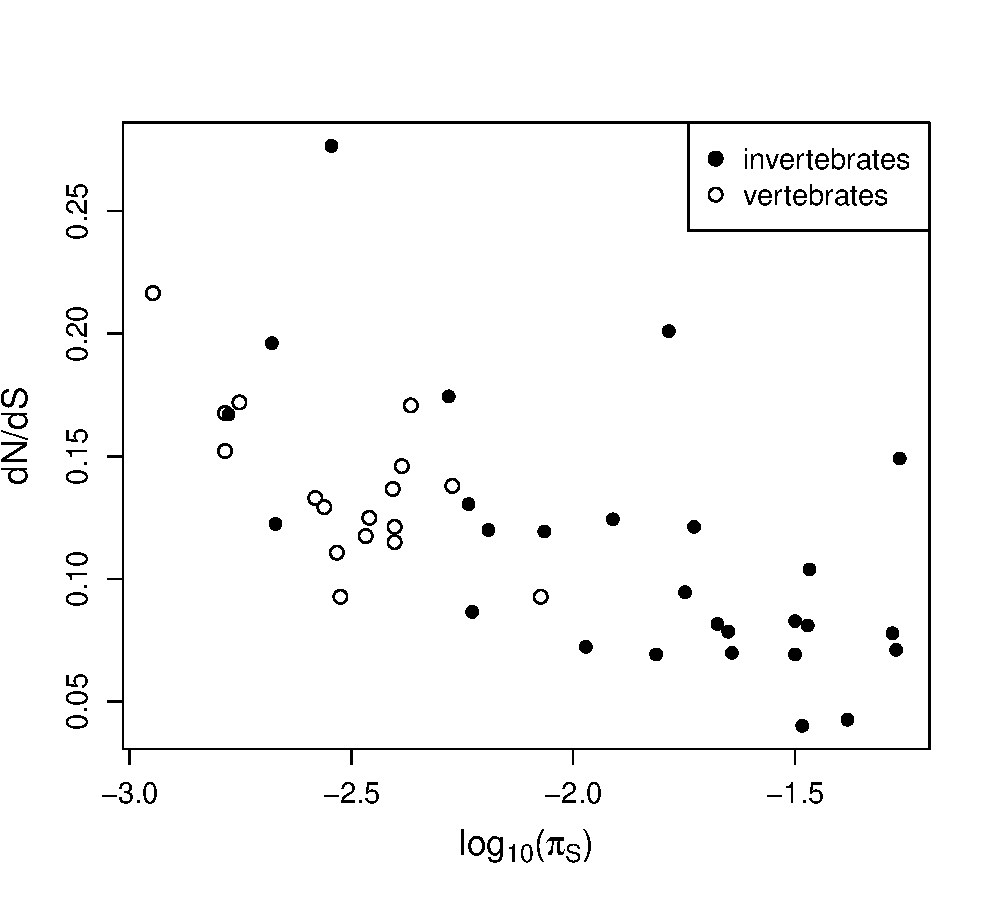
\includegraphics[width=0.8 \textwidth]{Journal_figs/drift_selection/Galtier_dNdS/Galtier_dNdS.pdf}
\end{center}
\caption{Data from 44 metazoan species. Each dot represents the
  average of over many genes plotting $\dNdS$ against synonymous
  diversity ($\pi_S$). Data from \citet{galtier2016adaptive} } \label{Galtier_dNdS}
\end{figure}

Across species, genome-wide averages of $\dNdS$ do seem to be
correlated with measures of the effective population size (such as
synonymous diversity), see Figure \ref{Galtier_dNdS}. This evidence supports the idea that in species with smaller effective
population sizes (lower $\pi_S$), proteins may be subject to lower degrees of
constraint, as very weakly deleterious mutations are able to fix. Thus,
some reasonable proportion of functional substitutions in populations
with small effective population sizes, such as humans, may be mildly deleterious.

\subsection{Appendix: A Sketch Proof of the probability of fixation of
weakly selected alleles} \label{Section:fixation_weakly_sel}
%Kolmogorov backward eqn. 1931
%Kimura, M. 1962 On the Probability of Fixation of Mutant Genes in a
%Population. for abitrary dominance in diffusion.

What is the probability a weakly beneficial or deleterious additive allele fixes in our population? \erin{I assume this is all using selection 1, 1+s/2 and 1+s, but you haven't explicitly specified your parameters for this case here. This result seems general to weakly beneficial or deleterious alleles but not clear that we're back to thinking about positively selected allele having benefit s and deleterious allele having a negative s} We'll let $P(\Delta p)$ be the probability that our allele frequency
shifts by $\Delta p$ in the next generation. Using this, we can write our probability $p_F(p)$ in terms of the probability of
achieving fixation averaged over the frequency in the next generation
\begin{equation}
p_F(p)  = \int p_F(p+\Delta p) P(\Delta p) d(\Delta p) \label{eqn:prob_fix_diff_step1}
\end{equation}
This is very similar to the technique that we used when deriving our
probability of escaping loss in a very large population above. \\

So we need an expression for $p_F(p+\Delta p)$. To obtain this, we'll
do a Taylor series expansion of $p_F(p)$, assuming that $\Delta p $ is small:
\begin{equation}
p_F(p+\Delta p) \approx p_F(p) + \Delta p \frac{dp_F(p)}{dp} + (\Delta p)^2
\frac{d^2p_F(p)}{dp^2} (p)
\end{equation}
ignoring higher order terms.\\

Taking the expectation over $\Delta p $ on both sides, as in
eqn. \ref{eqn:prob_fix_diff_step1}, we obtain
\begin{equation}
p_F(p) = p_F(p) + \E(\Delta p) \frac{dp_F (p)}{dp} + \E((\Delta p)^2)
\frac{d^2p_F(p)}{dp^2}
\end{equation}

Well, $\E(\Delta p) = \frac{s}{2}p(1-p)$ and $Var(\Delta p)= \E((\Delta
p)^2)-\E^2(\Delta p)$, so if $s \ll 1$ then $\E^2(\Delta p) \approx
0$, and $\E(\Delta p)^2 = \frac{p(1-p)}{2N}$. Substituting in these values and subtracting $p$ from both sides of our equation, this leaves us with
\begin{equation}
0= \frac{s}{2}p(1-p)\frac{dp_F (p) }{dp} + \frac{p(1-p)}{2N}
\frac{d^2p_F (p) }{dp^2}
\end{equation}
and we can specify the boundary conditions to be $p_F(1)=1$ and $p_F(0)=0$. 
Solving this differential equation is a somewhat involved process, but in
doing so we find that
\begin{equation}
p_F(p) = \frac{1-e^{-2Ns p }}{1-e^{-2Ns}}
\end{equation}
This proof can be extended
to alleles with arbitrary dominance, however, this does not lead to a
analytically tractable expression so we do not pursue this here. 

